% ==========================================
% LAMPIRAN C
% ==========================================
\cleardoublepage
\chapter{DOKUMENTASI LENGKAP EVALUASI DAN PENGUJIAN}
\label{chap:lampiran-c}

\section{Rincian \emph{Black-box Testing}}
\label{sec:c-blackbox}

Tabel~\ref{tab:c1-blackbox} berikut menyajikan rincian lengkap seluruh 20 skenario \emph{black-box testing} yang dilakukan pada modul \emph{People-to-Project}, mencakup skenario pengujian, ekspektasi keluaran, dan status hasil. Delapan belas skenario menghasilkan keluaran yang sesuai dengan ekspektasi yang telah ditetapkan, sementara dua skenario (TC15 dan TC16) berstatus Berhasil dengan Catatan.

\begin{longtable}{p{0.05\textwidth} p{0.17\textwidth} p{0.21\textwidth} p{0.27\textwidth} p{0.12\textwidth}}
\caption{Rincian \emph{Black-box Testing}} \label{tab:c1-blackbox} \\
\toprule
\textbf{Kode} & \textbf{\emph{Use Case}} & \textbf{Skenario} & \textbf{Ekspektasi Keluaran} & \textbf{Status} \\
\midrule
\endfirsthead
\multicolumn{5}{c}{\parbox{0.79\textwidth}{\centering \tablename\ \thetable\ Rincian \emph{Black-box Testing} (lanjutan)}} \\
\toprule
\textbf{Kode} & \textbf{\emph{Use Case}} & \textbf{Skenario} & \textbf{Ekspektasi Keluaran} & \textbf{Status} \\
\midrule
\endhead
\midrule
\multicolumn{5}{r}{\textit{Bersambung ke halaman berikutnya.}} \\
\endfoot
\bottomrule
\endlastfoot
TC01 & UC01 – \emph{Register} (\emph{Shared}) & Pengguna mengisi data registrasi valid & Akun berhasil dibuat; pengguna diarahkan ke halaman berikutnya & Berhasil \\
\midrule
TC02 & UC01 – \emph{Register} (\emph{Shared}) & Email sudah terdaftar & Sistem menampilkan pesan kesalahan bahwa email sudah digunakan & Berhasil \\
\midrule
TC03 & UC02 – \emph{Login} (\emph{Shared}) & Email dan kata sandi valid & Pengguna berhasil masuk; diarahkan ke halaman beranda aplikasi & Berhasil \\
\midrule
TC04 & UC02 – \emph{Login} (\emph{Shared}) & Kredensial tidak valid & Sistem menampilkan pesan kesalahan; pengguna tidak dapat masuk & Berhasil \\
\midrule
TC05 & UC03 – \emph{Logout} (\emph{Shared}) & Pengguna memilih keluar & Sesi pengguna diakhiri; pengguna diarahkan kembali ke halaman \emph{login} & Berhasil \\
\midrule
TC06 & UC04 – Kelola Profil Kolaboratif (\emph{Shared}) & Pengguna mengisi atau memperbarui 6 atribut profil kolaboratif (\emph{skill}, minat, pengalaman, gaya kerja, preferensi peran, ketersediaan waktu) & Profil berhasil disimpan; perubahan tercermin pada tampilan profil pengguna & Berhasil \\
\midrule
TC07 & UC05 – Melihat \emph{Feed} Rekomendasi & Profil pengguna lengkap & Sistem menampilkan daftar kegiatan yang diurutkan berdasarkan \emph{AffinityScore} tertinggi; kegiatan tanpa irisan waktu tidak muncul & Berhasil \\
\midrule
TC08 & UC05 – Melihat \emph{Feed} Rekomendasi & Profil pengguna belum lengkap & Sistem menampilkan pesan atau \emph{prompt} agar pengguna melengkapi profil terlebih dahulu; \emph{feed} tidak ditampilkan & Berhasil \\
\midrule
TC09 & UC05 – Melihat \emph{Feed} Rekomendasi & Suatu kegiatan tidak memiliki irisan slot waktu dengan pengguna & Kegiatan tersebut tidak muncul pada \emph{feed} pengguna (tersaring oleh \texttt{IsEligible}) & Berhasil \\
\midrule
TC10 & UC06 – Menyaring Rekomendasi & Pengguna menyaring \emph{feed} berdasarkan \emph{badge} (mis. ``hijau'') & \emph{Feed} hanya menampilkan kegiatan dengan \emph{badge} yang dipilih & Berhasil \\
\midrule
TC11 & UC06 – Menyaring Rekomendasi & Pengguna mengombinasikan filter atribut (minat, gaya kerja, preferensi peran) & \emph{Feed} menampilkan kegiatan yang sesuai dengan seluruh filter yang dipilih secara bersamaan & Berhasil \\
\midrule
TC12 & UC06 – Menyaring Rekomendasi & Kombinasi filter tidak menghasilkan kandidat & Sistem menampilkan tampilan kosong atau pesan bahwa tidak ada kegiatan yang sesuai filter & Berhasil \\
\midrule
TC13 & UC07 – Melihat Detail Kegiatan & Pengguna membuka salah satu kegiatan pada \emph{feed} & Sistem menampilkan halaman detail kegiatan beserta \emph{breakdown} kontribusi atribut (\emph{chip} kecocokan) & Berhasil \\
\midrule
TC14 & UC08 – Menyimpan Kegiatan & Pengguna menyimpan sebuah kegiatan & Kegiatan berhasil ditambahkan ke daftar simpanan; ikon simpan berubah menjadi aktif & Berhasil \\
\midrule
TC15 & UC09 – Membuat Kegiatan Baru & Pengguna mengisi seluruh \emph{field} kegiatan yang valid & Kegiatan berhasil dibuat dan muncul pada sistem; \emph{field} ``kategori'' yang tercantum dalam rancangan skenario telah digantikan mekanisme deteksi ikon otomatis berdasarkan kata kunci pada judul kegiatan & Berhasil dengan Catatan \\
\midrule
TC16 & UC09 – Membuat Kegiatan Baru & Pengguna mengirimkan formulir dengan \emph{field} wajib yang belum diisi & Sistem menampilkan pesan validasi; formulir tidak terkirim & Berhasil dengan Catatan \\
\midrule
TC17 & UC10 – Mendaftar ke Kegiatan & Pengguna mengajukan pendaftaran ke sebuah kegiatan & Pendaftaran berhasil terkirim; status berubah menjadi \emph{Pending} & Berhasil \\
\midrule
TC18 & UC10 – Mendaftar ke Kegiatan & Pengguna membatalkan pendaftaran yang masih \emph{Pending} & Pendaftaran berhasil dibatalkan; status kembali ke kondisi awal & Berhasil \\
\midrule
TC19 & UC11 – Mengelola Pendaftar & Pembuat kegiatan menerima seorang pendaftar & Pendaftar berhasil diterima; status pendaftaran berubah menjadi Diterima & Berhasil \\
\midrule
TC20 & UC11 – Mengelola Pendaftar & Pembuat kegiatan menolak seorang pendaftar & Pendaftar ditolak; status pendaftaran berubah menjadi Ditolak & Berhasil \\
\end{longtable}

Catatan: TC15 dan TC16 berstatus Berhasil dengan Catatan karena fungsionalitas inti pembuatan kegiatan terbukti berjalan benar, namun \emph{field} ``kategori'' yang tercantum pada rancangan skenario telah digantikan mekanisme deteksi ikon otomatis berdasarkan kata kunci pada judul kegiatan dalam implementasi saat ini. Penyesuaian ini bersifat teknis dan tidak memengaruhi alur utama.

\section{Rincian Evaluasi Algoritma \emph{AffinityEngine}}
\label{sec:c-evaluasi-algo}

Tabel~\ref{tab:c2-algo} berikut menyajikan rincian lengkap seluruh 14 skenario evaluasi algoritma \emph{AffinityEngine}, mencakup komponen yang diuji, skenario pengujian, dan ekspektasi nilai keluaran berdasarkan rumus yang dirancang pada Bab IV. Seluruh skenario diverifikasi dengan membandingkan hasil perhitungan manual terhadap hasil sistem, dan seluruhnya menghasilkan nilai yang sesuai.

\begin{longtable}{p{0.05\textwidth} p{0.15\textwidth} p{0.23\textwidth} p{0.31\textwidth} p{0.08\textwidth}}
\caption{Rincian Evaluasi Algoritma \emph{AffinityEngine}} \label{tab:c2-algo} \\
\toprule
\textbf{Kode} & \textbf{Komponen} & \textbf{Skenario} & \textbf{Ekspektasi Keluaran} & \textbf{Status} \\
\midrule
\endfirsthead
\multicolumn{5}{c}{\parbox{0.79\textwidth}{\centering \tablename\ \thetable\ Rincian Evaluasi Algoritma \emph{AffinityEngine} (lanjutan)}} \\
\toprule
\textbf{Kode} & \textbf{Komponen} & \textbf{Skenario} & \textbf{Ekspektasi Keluaran} & \textbf{Status} \\
\midrule
\endhead
\midrule
\multicolumn{5}{r}{\textit{Bersambung ke halaman berikutnya.}} \\
\endfoot
\bottomrule
\endlastfoot
AL01 & Skor \emph{Skill} & Profil memiliki semua \emph{skill} yang dibutuhkan kegiatan (2 dari 2 cocok) & Skor \emph{skill} $= 2/2 = 1{,}00$ & Berhasil \\
\midrule
AL02 & Skor \emph{Skill} & Profil memiliki sebagian \emph{skill} yang dibutuhkan (1 dari 2 cocok) & Skor \emph{skill} $= 1/2 = 0{,}50$ & Berhasil \\
\midrule
AL03 & Skor \emph{Skill} & Tidak ada \emph{skill} profil yang cocok dengan kebutuhan kegiatan (0 dari 2) & Skor \emph{skill} $= 0/2 = 0{,}00$ & Berhasil \\
\midrule
AL04 & Skor \emph{Skill} & Kegiatan tidak mensyaratkan \emph{skill} spesifik (tidak ada persyaratan) & Skor \emph{skill} $= 1{,}00$ (skor penuh; tidak ada tuntutan) & Berhasil \\
\midrule
AL05 & Skor Pengalaman & Level pengalaman profil dan kegiatan sama (selisih $= 0$) & Skor pengalaman $= 1 - |0|/2 = 1{,}00$ & Berhasil \\
\midrule
AL06 & Skor Pengalaman & Level pengalaman berselisih 1 tingkat & Skor pengalaman $= 1 - 1/2 = 0{,}50$ & Berhasil \\
\midrule
AL07 & Skor Pengalaman & Level pengalaman berselisih 2 tingkat (selisih maksimum pada skala 1--3) & Skor pengalaman $= 1 - 2/2 = 0{,}00$ & Berhasil \\
\midrule
AL08 & Skor Minat & Seluruh \emph{tag} minat kegiatan tercakup dalam minat profil (2 dari 2 \emph{tag}) & Skor minat $= 2/2 = 1{,}00$ & Berhasil \\
\midrule
AL09 & Skor Minat & Sebagian \emph{tag} minat kegiatan tercakup dalam minat profil (2 dari 3 \emph{tag}) & Skor minat $= 2/3 \approx 0{,}667$ & Berhasil \\
\midrule
AL10 & Skor Gaya Kerja & Gaya kerja profil dan kegiatan sama (\texttt{"Terstruktur"}) & Skor gaya kerja $= 1{,}00$ & Berhasil \\
\midrule
AL11 & Skor Gaya Kerja & Gaya kerja profil dan kegiatan berbeda & Skor gaya kerja $= 0{,}00$ & Berhasil \\
\midrule
AL12 & Skor Preferensi Peran & Preferensi peran profil cocok dengan salah satu peran yang dibutuhkan kegiatan & Skor peran $= 1{,}00$ & Berhasil \\
\midrule
AL13 & Skor Preferensi Peran & Preferensi peran profil tidak cocok dengan peran yang dibutuhkan kegiatan & Skor peran $= 0{,}00$ & Berhasil \\
\midrule
AL14 & Skor Preferensi Peran & Kegiatan tidak menetapkan peran spesifik ($|\text{peran}| = 0$) & Skor peran $= 0{,}50$ (netral; tidak ada tuntutan peran) & Berhasil \\
\end{longtable}

\section{Rincian \emph{User Acceptance Test} (UAT)}
\label{sec:c-uat}

UAT dilakukan terhadap sepuluh responden mahasiswa yang mencoba skenario penggunaan utama modul \emph{People-to-Project} secara langsung. Responden memberikan penilaian terhadap delapan pernyataan menggunakan skala Likert 1 sampai 5. Rata-rata skor per aspek kemudian dikonversi ke persentase dan dikategorikan berdasarkan ambang batas penerimaan: Sangat Diterima ($\geq$80\%), Diterima ($\geq$60\%), Cukup Diterima ($\geq$40\%), Tidak Diterima ($\geq$20\%), dan Sangat Tidak Diterima ($<$20\%).

Tabel~\ref{tab:c3-uat} menyajikan rincian rata-rata skor dan kategori penerimaan untuk setiap aspek yang dinilai.

\begin{longtable}{p{0.04\textwidth} p{0.17\textwidth} p{0.27\textwidth} p{0.09\textwidth} p{0.08\textwidth} p{0.12\textwidth}}
\caption{Rincian Hasil \emph{User Acceptance Test} (UAT)} \label{tab:c3-uat} \\
\toprule
\textbf{No.} & \textbf{Aspek yang Dinilai} & \textbf{Pernyataan UAT} & \textbf{Rata-rata Skor} & \textbf{Persen-tase} & \textbf{Kategori Penerimaan} \\
\midrule
\endfirsthead
\multicolumn{6}{c}{\parbox{0.75\textwidth}{\centering \tablename\ \thetable\ Rincian Hasil UAT (lanjutan)}} \\
\toprule
\textbf{No.} & \textbf{Aspek yang Dinilai} & \textbf{Pernyataan UAT} & \textbf{Rata-rata Skor} & \textbf{Persen-tase} & \textbf{Kategori Penerimaan} \\
\midrule
\endhead
\midrule
\multicolumn{6}{r}{\textit{Bersambung ke halaman berikutnya.}} \\
\endfoot
\bottomrule
\endlastfoot
1 & Pengelolaan profil kolaboratif & Sistem membantu saya mengisi dan memperbarui profil kolaboratif, meliputi minat, \emph{skill}, pengalaman, gaya kerja, dan preferensi peran. & 4{,}1 & 82\% & Diterima \\
\midrule
2 & \emph{Feed} rekomendasi kegiatan & Sistem membantu saya menemukan kegiatan kolaboratif yang sesuai dengan profil saya. & 3{,}7 & 74\% & Diterima \\
\midrule
3 & \emph{Badge} kecocokan & \emph{Badge} tingkat kecocokan, yaitu hijau, kuning, dan abu-abu, membantu saya menilai relevansi suatu kegiatan secara cepat. & 4{,}2 & 84\% & Sangat Diterima \\
\midrule
4 & \emph{Breakdown} kontribusi atribut & Rincian kontribusi atribut dalam bentuk \emph{chip} membantu saya memahami alasan suatu kegiatan direkomendasikan. & 3{,}9 & 78\% & Diterima \\
\midrule
5 & Detail kegiatan kolaboratif & Informasi detail kegiatan, seperti deskripsi, \emph{role} yang dibutuhkan, kuota, dan \emph{timeline}, mudah dipahami. & 4{,}1 & 82\% & Diterima \\
\midrule
6 & Pendaftaran ke kegiatan & Proses mengajukan pendaftaran ke kegiatan kolaboratif mudah dilakukan. & 4{,}2 & 84\% & Sangat Diterima \\
\midrule
7 & Pembuatan kegiatan & Fitur membuat kegiatan baru membantu pengguna yang ingin mencari anggota atau kolaborator. & 4{,}0 & 80\% & Diterima \\
\midrule
8 & Pengelolaan pendaftar & Fitur melihat dan memproses pendaftar membantu pembuat kegiatan mengelola calon anggota. & 4{,}0 & 80\% & Diterima \\
\end{longtable}

\section{Rincian Skor \emph{System Usability Scale} (SUS) per Butir}
\label{sec:c-sus}

SUS dilakukan terhadap sepuluh responden yang sama dengan UAT. Tabel~\ref{tab:c4-sus} menyajikan rincian rata-rata skor mentah per butir beserta nilai kontribusi masing-masing. Pernyataan bernomor ganjil bersifat positif (kontribusi $=$ skor $- 1$) dan bernomor genap bersifat negatif (kontribusi $= 5 -$ skor). Total kontribusi dikalikan 2,5 menghasilkan skor SUS akhir.

\begin{longtable}{p{0.05\textwidth} p{0.45\textwidth} p{0.09\textwidth} p{0.11\textwidth} p{0.12\textwidth}}
\caption{Rincian Skor \emph{System Usability Scale} (SUS) per Butir} \label{tab:c4-sus} \\
\toprule
\textbf{No.} & \textbf{Pernyataan SUS} & \textbf{Sifat} & \textbf{Rata-rata Skor} & \textbf{Rata-rata Kontribusi} \\
\midrule
\endfirsthead
\multicolumn{5}{c}{\parbox{0.79\textwidth}{\centering \tablename\ \thetable\ Rincian Skor SUS per Butir (lanjutan)}} \\
\toprule
\textbf{No.} & \textbf{Pernyataan SUS} & \textbf{Sifat} & \textbf{Rata-rata Skor} & \textbf{Rata-rata Kontribusi} \\
\midrule
\endhead
\midrule
\multicolumn{5}{r}{\textit{Bersambung ke halaman berikutnya.}} \\
\endfoot
\bottomrule
\endlastfoot
1 & Saya merasa akan sering menggunakan sistem aplikasi kolaborasi ini ketika ingin mencari atau bergabung dengan kegiatan kolaboratif. & Positif & 3{,}7 & 2{,}7 \\
\midrule
2 & Saya merasa sistem aplikasi kolaborasi ini terlalu rumit untuk digunakan. & Negatif & 2{,}5 & 2{,}5 \\
\midrule
3 & Saya merasa sistem aplikasi kolaborasi ini mudah digunakan. & Positif & 3{,}4 & 2{,}4 \\
\midrule
4 & Saya merasa membutuhkan bantuan orang lain untuk dapat menggunakan sistem ini. & Negatif & 3{,}3 & 1{,}7 \\
\midrule
5 & Saya merasa fitur-fitur dalam sistem ini terintegrasi dengan baik. & Positif & 3{,}4 & 2{,}4 \\
\midrule
6 & Saya merasa terdapat terlalu banyak ketidakkonsistenan dalam sistem ini. & Negatif & 2{,}8 & 2{,}2 \\
\midrule
7 & Saya merasa sebagian besar mahasiswa akan cepat memahami cara menggunakan sistem ini. & Positif & 3{,}6 & 2{,}6 \\
\midrule
8 & Saya merasa sistem ini membingungkan untuk digunakan. & Negatif & 2{,}1 & 2{,}9 \\
\midrule
9 & Saya merasa percaya diri saat menggunakan sistem ini. & Positif & 3{,}9 & 2{,}9 \\
\midrule
10 & Saya perlu mempelajari banyak hal terlebih dahulu sebelum dapat menggunakan sistem ini. & Negatif & 2{,}8 & 2{,}2 \\
\midrule
\multicolumn{4}{r}{\textbf{Total Kontribusi (24{,}5) $\times$ 2{,}5}} & \textbf{61{,}25} \\
\end{longtable}

\section{Dokumentasi Visual Hasil Kuesioner}
\label{sec:c-visual}

Subbab ini menyajikan visualisasi distribusi jawaban responden untuk seluruh butir kuesioner evaluasi eksternal, mencakup delapan aspek \emph{User Acceptance Test} (UAT) modul \emph{People-to-Project} dan sepuluh butir \emph{System Usability Scale} (SUS).

\subsection{Distribusi Jawaban UAT Modul \emph{People-to-Project}}
\label{subsec:c-visual-uat}

Gambar~\ref{fig:c-uat1} hingga Gambar~\ref{fig:c-uat8} menyajikan distribusi jawaban responden untuk delapan aspek UAT modul \emph{People-to-Project}.

\begin{figure}[H]
  \centering
  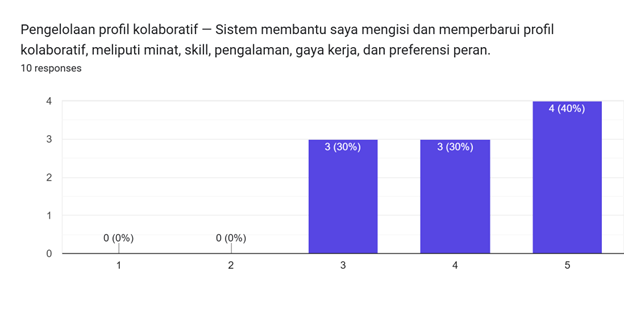
\includegraphics[width=0.85\textwidth]{images/UAT/UAT1}
  \caption{Distribusi Jawaban Aspek Pengelolaan Profil Kolaboratif}
  \label{fig:c-uat1}
\end{figure}

\begin{figure}[H]
  \centering
  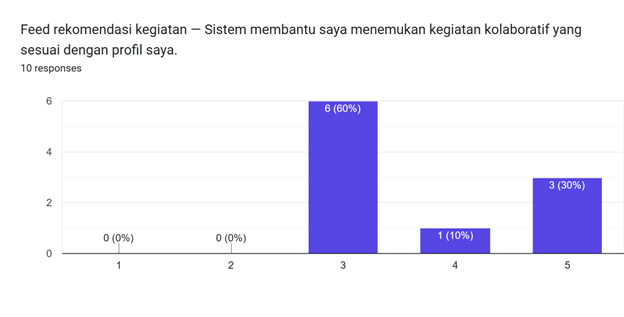
\includegraphics[width=0.85\textwidth]{images/UAT/UAT2}
  \caption{Distribusi Jawaban Aspek \emph{Feed} Rekomendasi Kegiatan}
  \label{fig:c-uat2}
\end{figure}

\begin{figure}[H]
  \centering
  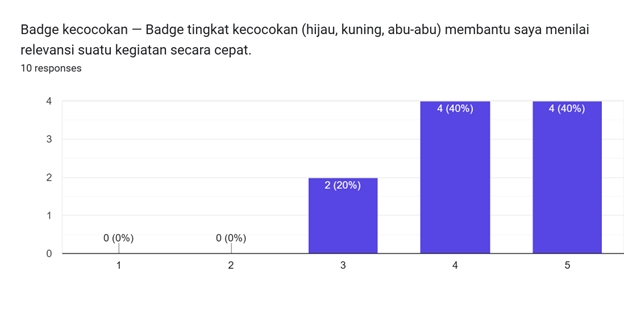
\includegraphics[width=0.85\textwidth]{images/UAT/UAT3}
  \caption{Distribusi Jawaban Aspek \emph{Badge} Kecocokan}
  \label{fig:c-uat3}
\end{figure}

\begin{figure}[H]
  \centering
  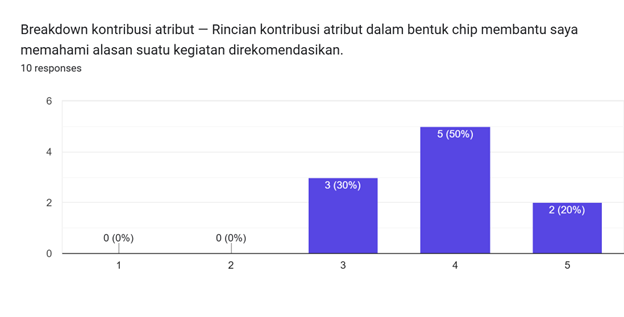
\includegraphics[width=0.85\textwidth]{images/UAT/UAT4}
  \caption{Distribusi Jawaban Aspek \emph{Breakdown} Kontribusi Atribut}
  \label{fig:c-uat4}
\end{figure}

\begin{figure}[H]
  \centering
  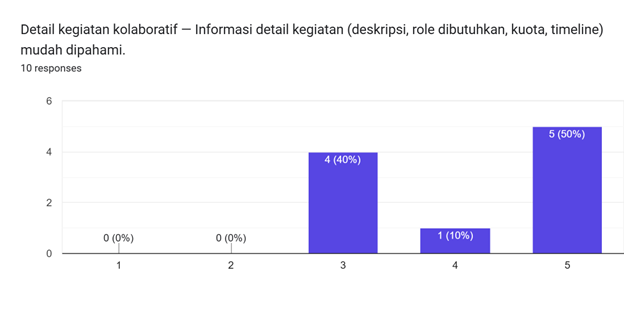
\includegraphics[width=0.85\textwidth]{images/UAT/UAT5}
  \caption{Distribusi Jawaban Aspek Detail Kegiatan Kolaboratif}
  \label{fig:c-uat5}
\end{figure}

\begin{figure}[H]
  \centering
  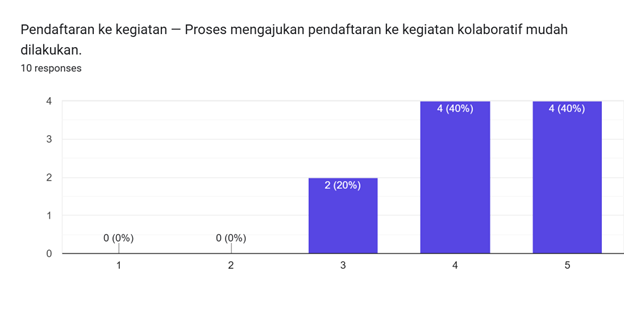
\includegraphics[width=0.85\textwidth]{images/UAT/UAT6}
  \caption{Distribusi Jawaban Aspek Pendaftaran ke Kegiatan}
  \label{fig:c-uat6}
\end{figure}

\begin{figure}[H]
  \centering
  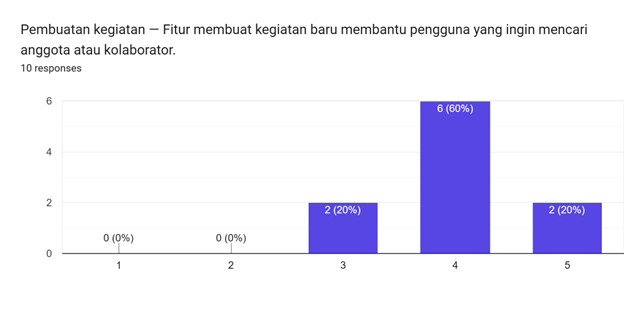
\includegraphics[width=0.85\textwidth]{images/UAT/UAT7}
  \caption{Distribusi Jawaban Aspek Pembuatan Kegiatan}
  \label{fig:c-uat7}
\end{figure}

\begin{figure}[H]
  \centering
  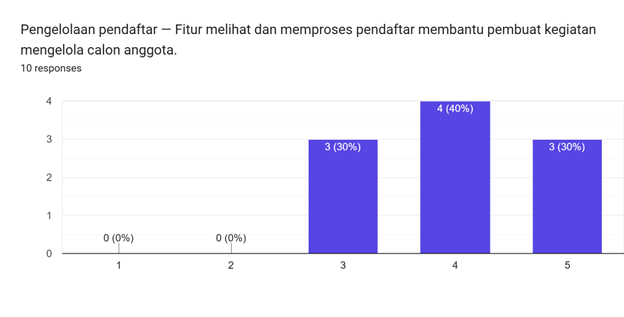
\includegraphics[width=0.85\textwidth]{images/UAT/UAT8}
  \caption{Distribusi Jawaban Aspek Pengelolaan Pendaftar}
  \label{fig:c-uat8}
\end{figure}

\subsection{Distribusi Jawaban SUS}
\label{subsec:c-visual-sus}

Gambar~\ref{fig:c-sus1} hingga Gambar~\ref{fig:c-sus10} menyajikan distribusi jawaban responden untuk sepuluh butir SUS.

\begin{figure}[H]
  \centering
  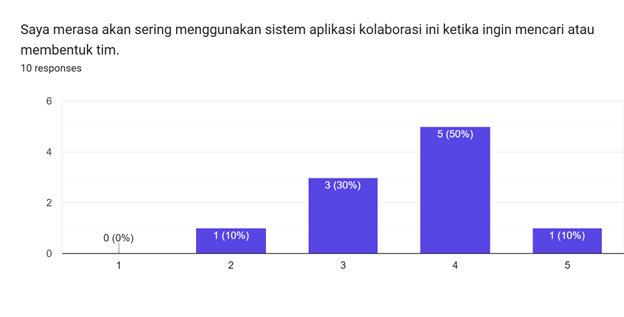
\includegraphics[width=0.85\textwidth]{images/SUS/SUS1}
  \caption{Distribusi Jawaban Butir SUS-1 (Sering Menggunakan)}
  \label{fig:c-sus1}
\end{figure}

\begin{figure}[H]
  \centering
  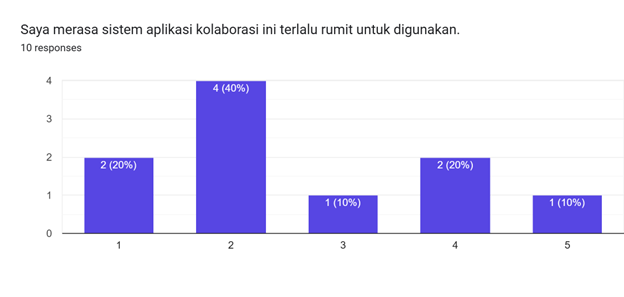
\includegraphics[width=0.85\textwidth]{images/SUS/SUS2}
  \caption{Distribusi Jawaban Butir SUS-2 (Terlalu Rumit)}
  \label{fig:c-sus2}
\end{figure}

\begin{figure}[H]
  \centering
  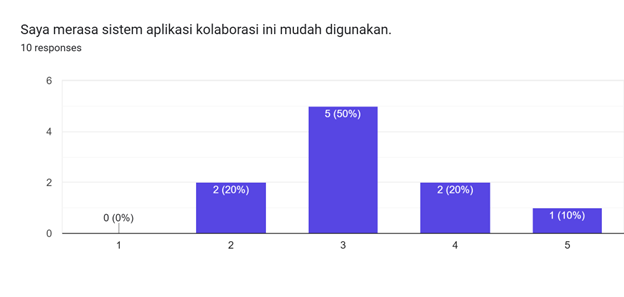
\includegraphics[width=0.85\textwidth]{images/SUS/SUS3}
  \caption{Distribusi Jawaban Butir SUS-3 (Mudah Digunakan)}
  \label{fig:c-sus3}
\end{figure}

\begin{figure}[H]
  \centering
  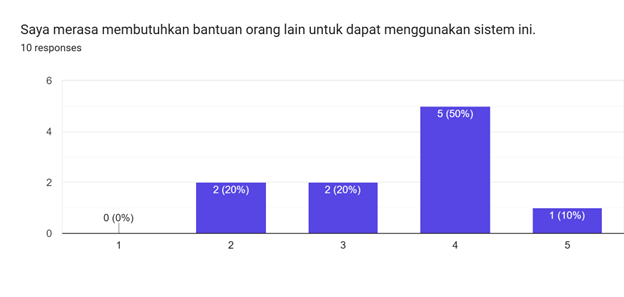
\includegraphics[width=0.85\textwidth]{images/SUS/SUS4}
  \caption{Distribusi Jawaban Butir SUS-4 (Butuh Bantuan Orang Lain)}
  \label{fig:c-sus4}
\end{figure}

\begin{figure}[H]
  \centering
  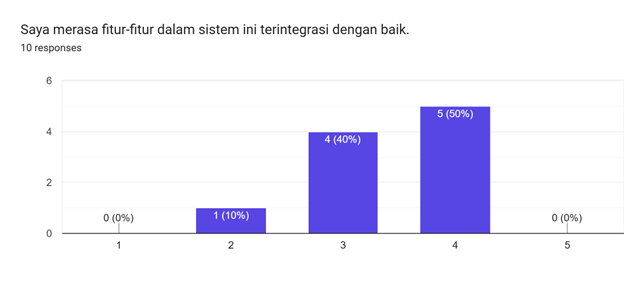
\includegraphics[width=0.85\textwidth]{images/SUS/SUS5}
  \caption{Distribusi Jawaban Butir SUS-5 (Fitur Terintegrasi)}
  \label{fig:c-sus5}
\end{figure}

\begin{figure}[H]
  \centering
  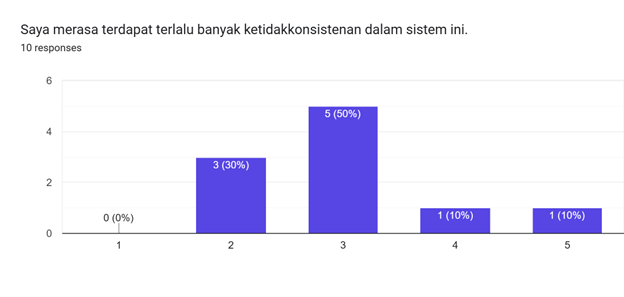
\includegraphics[width=0.85\textwidth]{images/SUS/SUS6}
  \caption{Distribusi Jawaban Butir SUS-6 (Ketidakkonsistenan)}
  \label{fig:c-sus6}
\end{figure}

\begin{figure}[H]
  \centering
  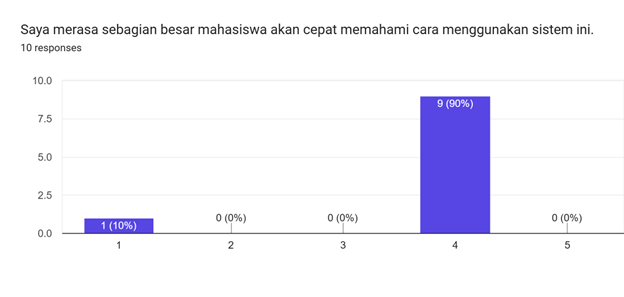
\includegraphics[width=0.85\textwidth]{images/SUS/SUS7}
  \caption{Distribusi Jawaban Butir SUS-7 (Cepat Dipahami)}
  \label{fig:c-sus7}
\end{figure}

\begin{figure}[H]
  \centering
  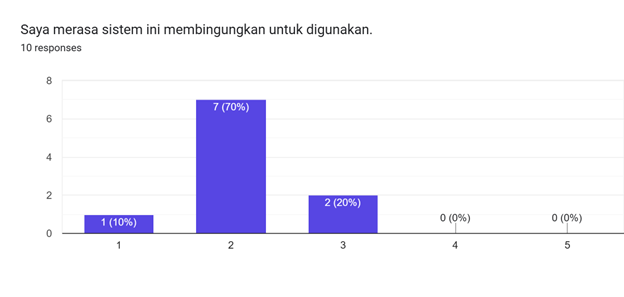
\includegraphics[width=0.85\textwidth]{images/SUS/SUS8}
  \caption{Distribusi Jawaban Butir SUS-8 (Membingungkan)}
  \label{fig:c-sus8}
\end{figure}

\begin{figure}[H]
  \centering
  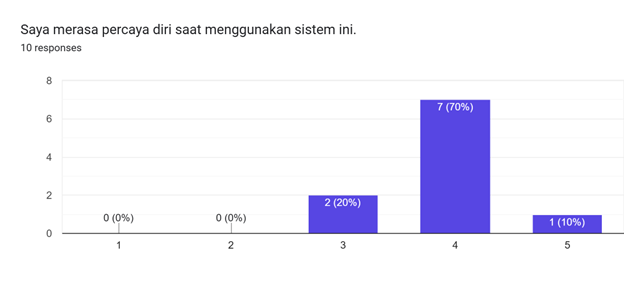
\includegraphics[width=0.85\textwidth]{images/SUS/SUS9}
  \caption{Distribusi Jawaban Butir SUS-9 (Percaya Diri)}
  \label{fig:c-sus9}
\end{figure}

\begin{figure}[H]
  \centering
  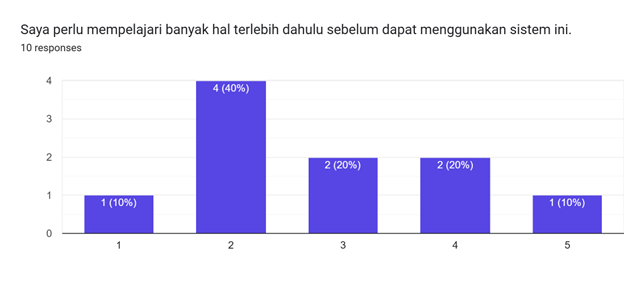
\includegraphics[width=0.85\textwidth]{images/SUS/SUS10}
  \caption{Distribusi Jawaban Butir SUS-10 (Perlu Mempelajari)}
  \label{fig:c-sus10}
\end{figure}

\section{Dokumentasi Pelaksanaan UAT dan SUS}
\label{sec:c-dok-uat}

UAT dan SUS dilaksanakan secara tatap muka maupun daring dengan melibatkan sepuluh responden mahasiswa aktif yang sama. Tabel~\ref{tab:c5-responden} menyajikan daftar responden yang berpartisipasi dalam kedua sesi pengujian tersebut.

\begin{table}[H]
  \caption{Profil Responden UAT dan SUS}
  \label{tab:c5-responden}
  \begin{tabularx}{\textwidth}{p{0.07\textwidth} p{0.25\textwidth} p{0.35\textwidth} X}
    \toprule
    \textbf{No.} & \textbf{Kode} & \textbf{Asal Kampus} & \textbf{Dok.} \\
    \midrule
    1 & Responden 1 & Institut Teknologi Bandung & Gambar~\ref{fig:c-dok1} \\
    \midrule
    2 & Responden 2 & Institut Teknologi Bandung & Gambar~\ref{fig:c-dok2} \\
    \midrule
    3 & Responden 3 & Institut Teknologi Bandung & Gambar~\ref{fig:c-dok3} \\
    \midrule
    4 & Responden 4 & Institut Teknologi Bandung & Gambar~\ref{fig:c-dok4} \\
    \midrule
    5 & Responden 5 & Institut Teknologi Bandung & Gambar~\ref{fig:c-dok5} \\
    \midrule
    6 & Responden 6 & Institut Teknologi Bandung & Gambar~\ref{fig:c-dok6} \\
    \midrule
    7 & Responden 7 & Institut Teknologi Bandung & Gambar~\ref{fig:c-dok6} \\
    \midrule
    8 & Responden 8 & Institut Teknologi Bandung & Gambar~\ref{fig:c-dok7} \\
    \midrule
    9 & Responden 9 & Institut Teknologi Bandung & Gambar~\ref{fig:c-dok7} \\
    \midrule
    10 & Responden 10 & Institut Teknologi Bandung & Gambar~\ref{fig:c-dok8} \\
    \bottomrule
  \end{tabularx}
\end{table}

\begin{figure}[H]
  \centering
  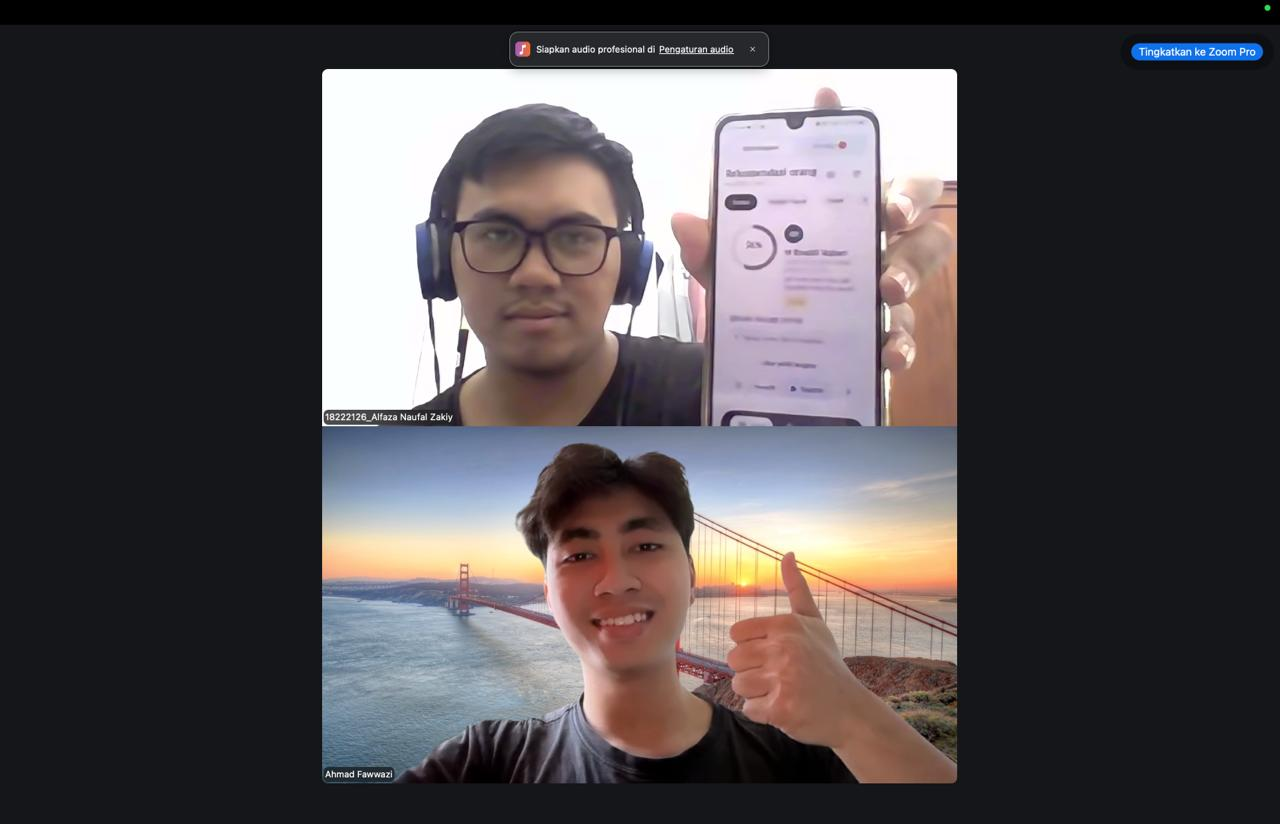
\includegraphics[width=0.75\textwidth]{images/Responden/R1}
  \caption{Dokumentasi Sesi Pengujian bersama Responden 1}
  \label{fig:c-dok1}
\end{figure}

\begin{figure}[H]
  \centering
  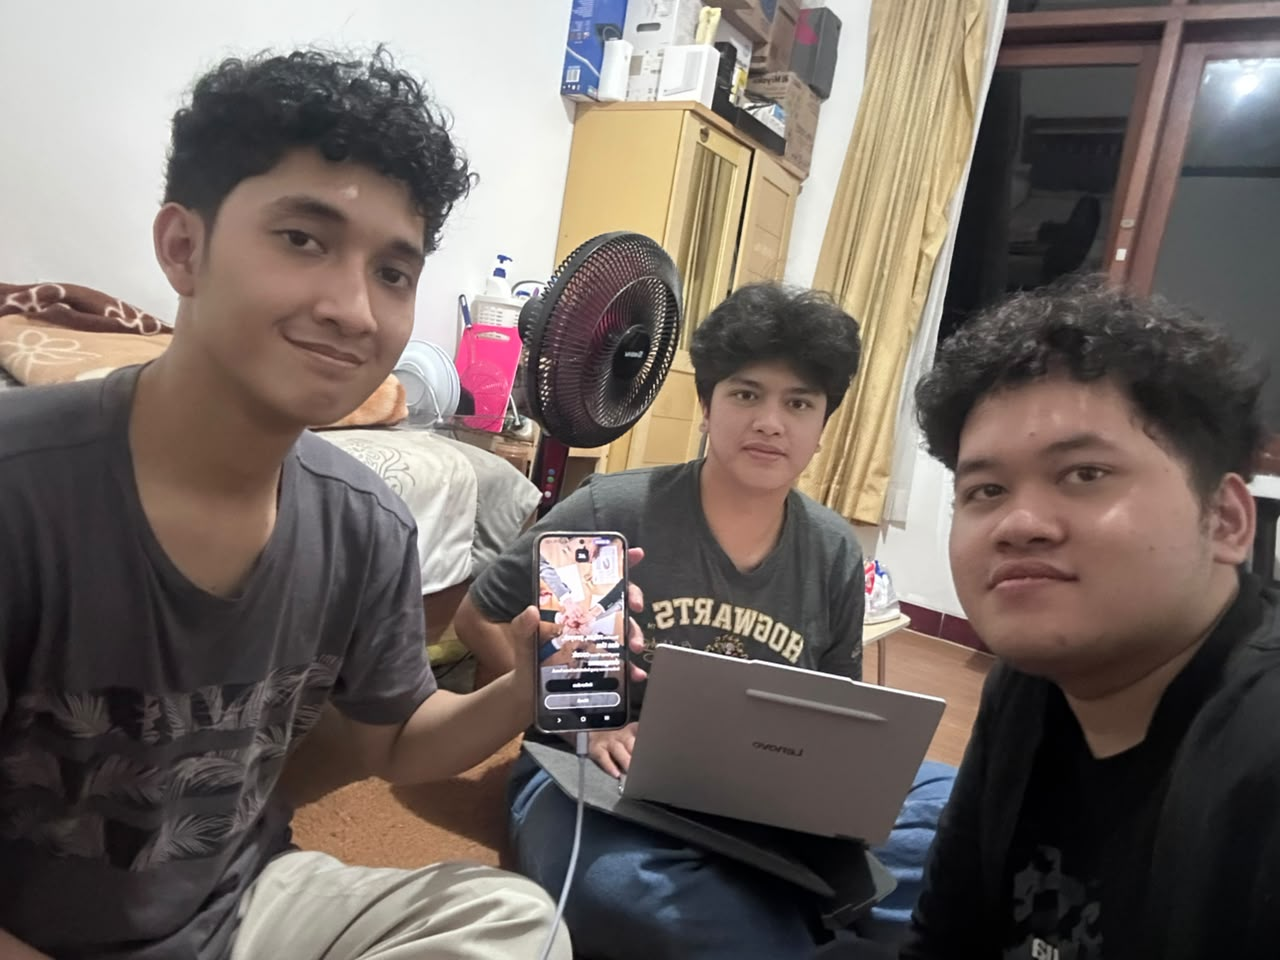
\includegraphics[width=0.75\textwidth]{images/Responden/R2}
  \caption{Dokumentasi Sesi Pengujian bersama Responden 2}
  \label{fig:c-dok2}
\end{figure}

\begin{figure}[H]
  \centering
  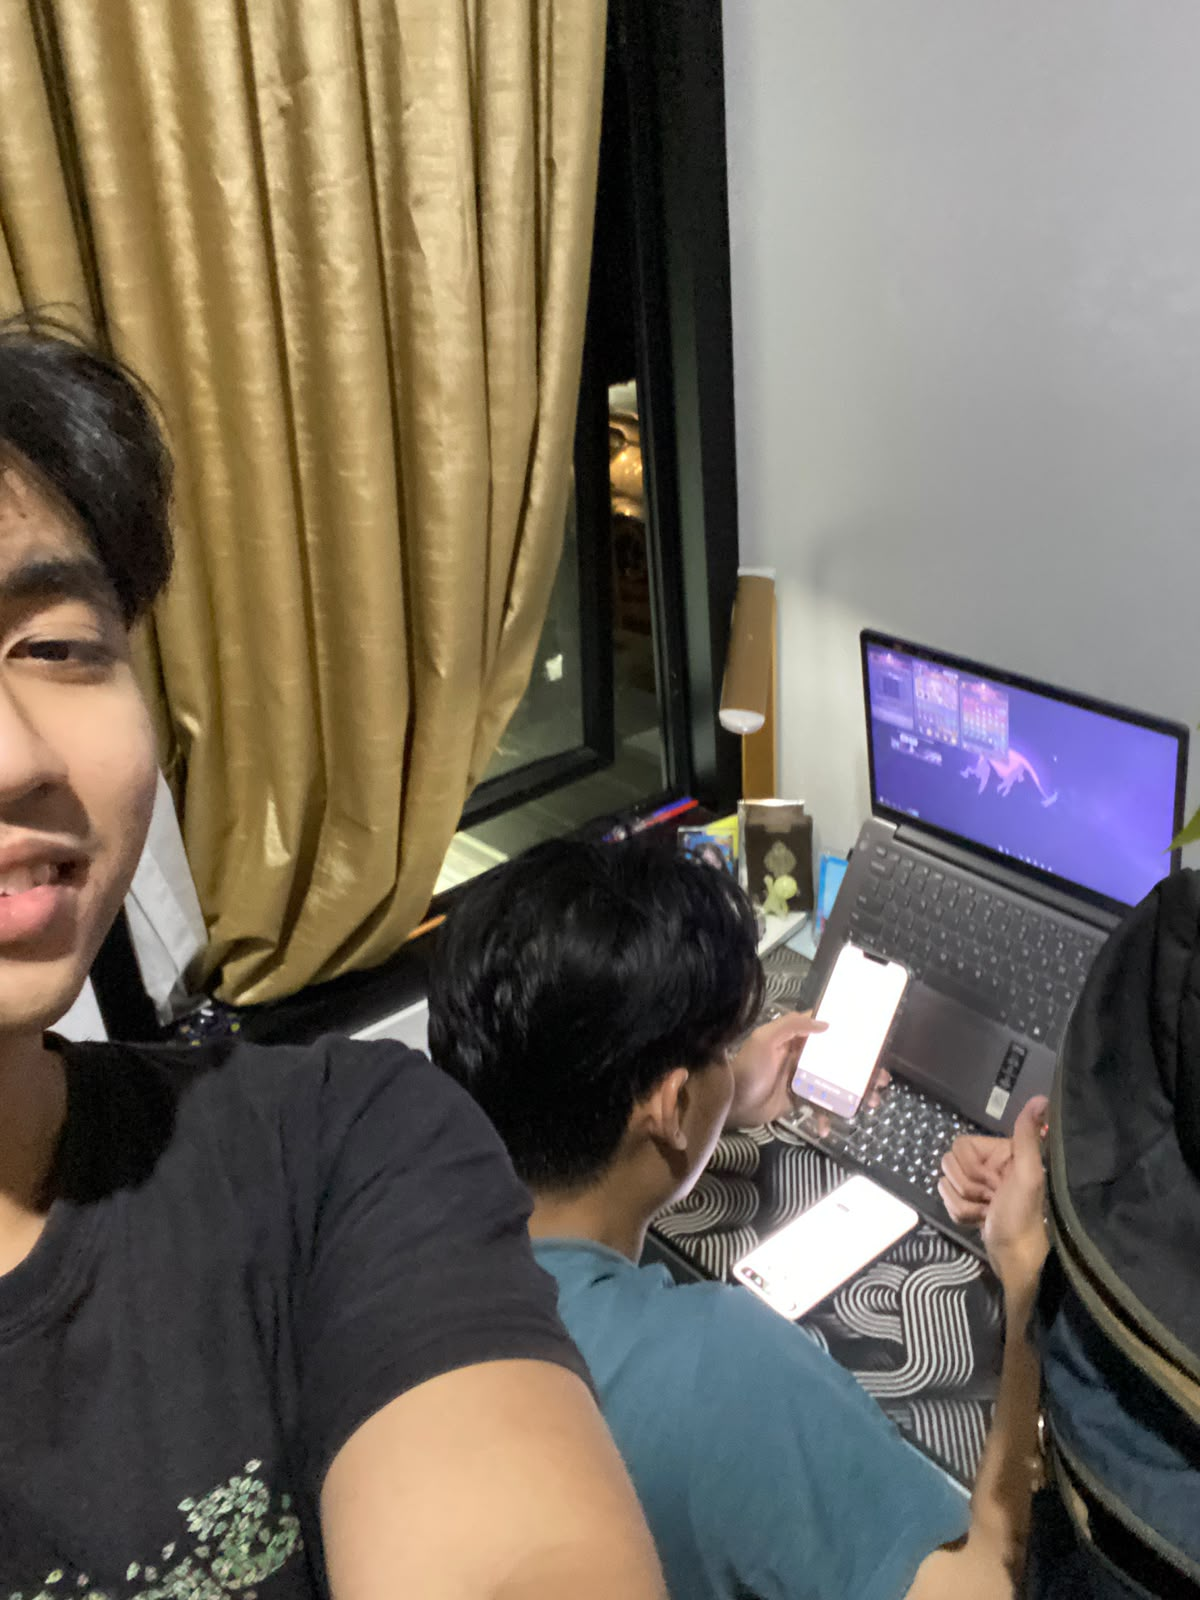
\includegraphics[width=0.75\textwidth]{images/Responden/R3}
  \caption{Dokumentasi Sesi Pengujian bersama Responden 3}
  \label{fig:c-dok3}
\end{figure}

\begin{figure}[H]
  \centering
  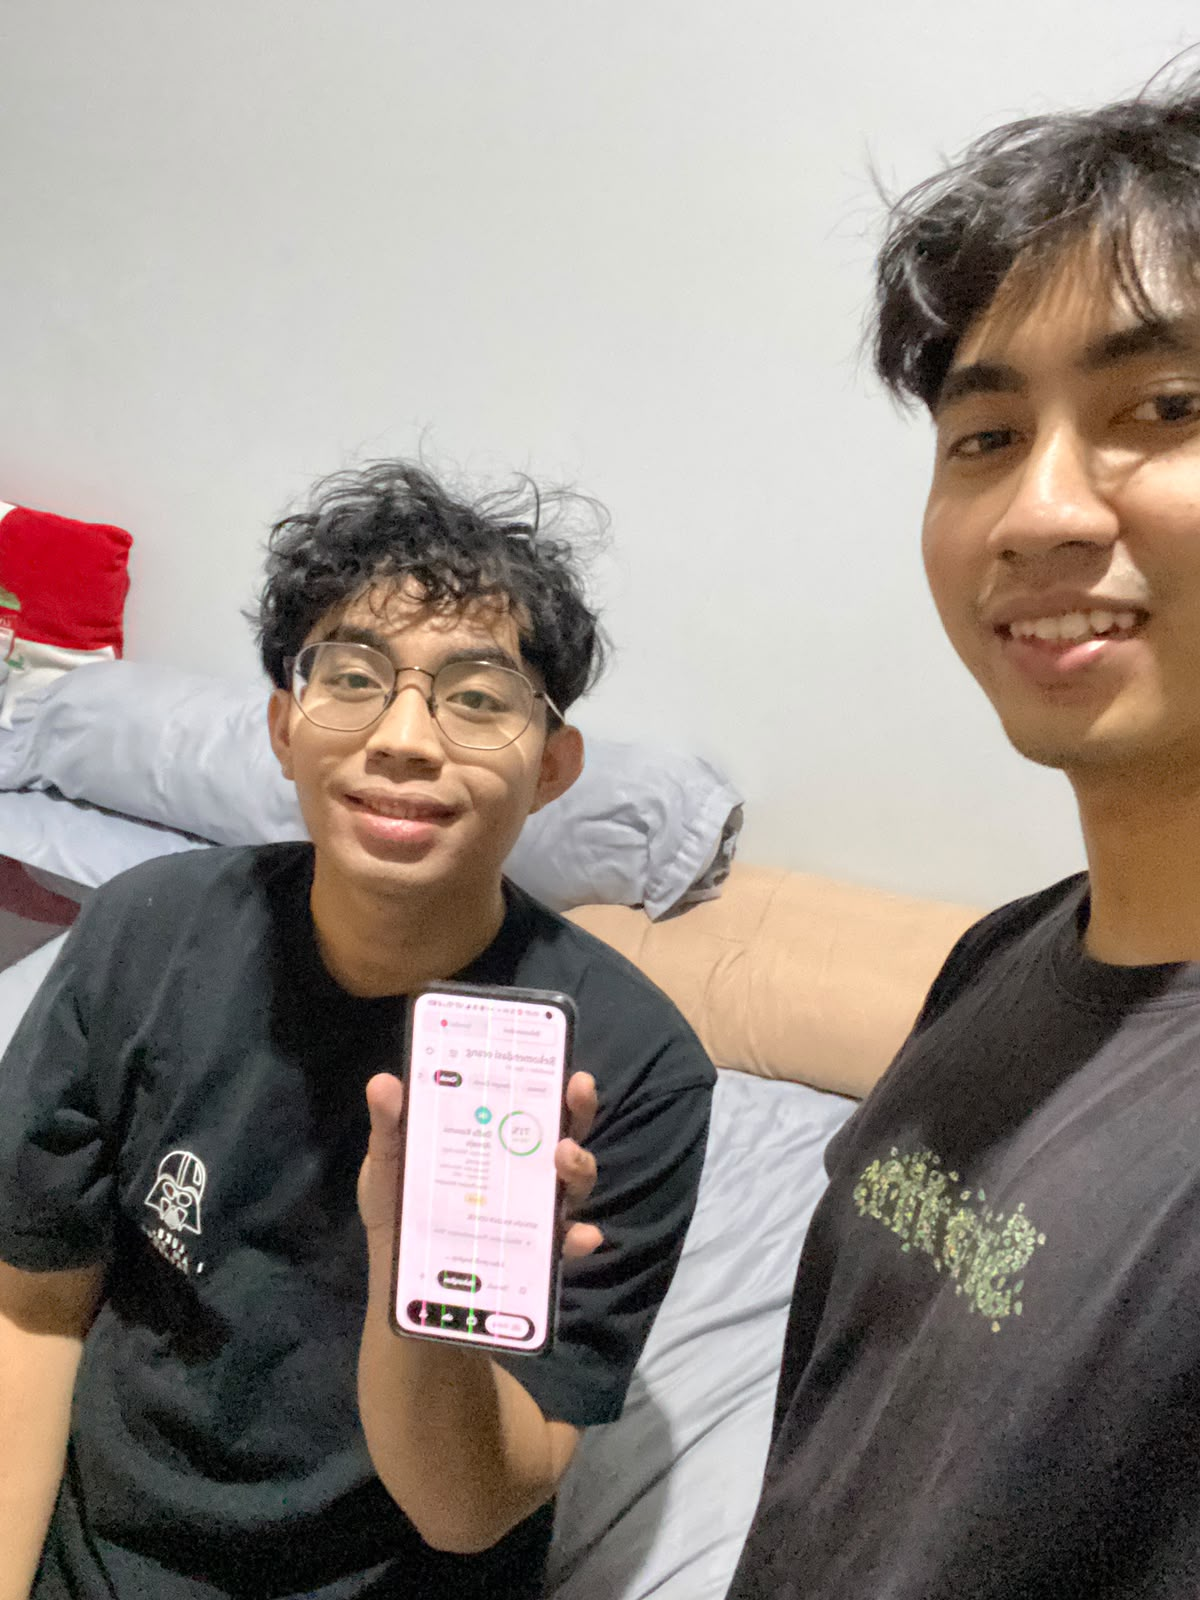
\includegraphics[width=0.75\textwidth]{images/Responden/R4}
  \caption{Dokumentasi Sesi Pengujian bersama Responden 4}
  \label{fig:c-dok4}
\end{figure}

\begin{figure}[H]
  \centering
  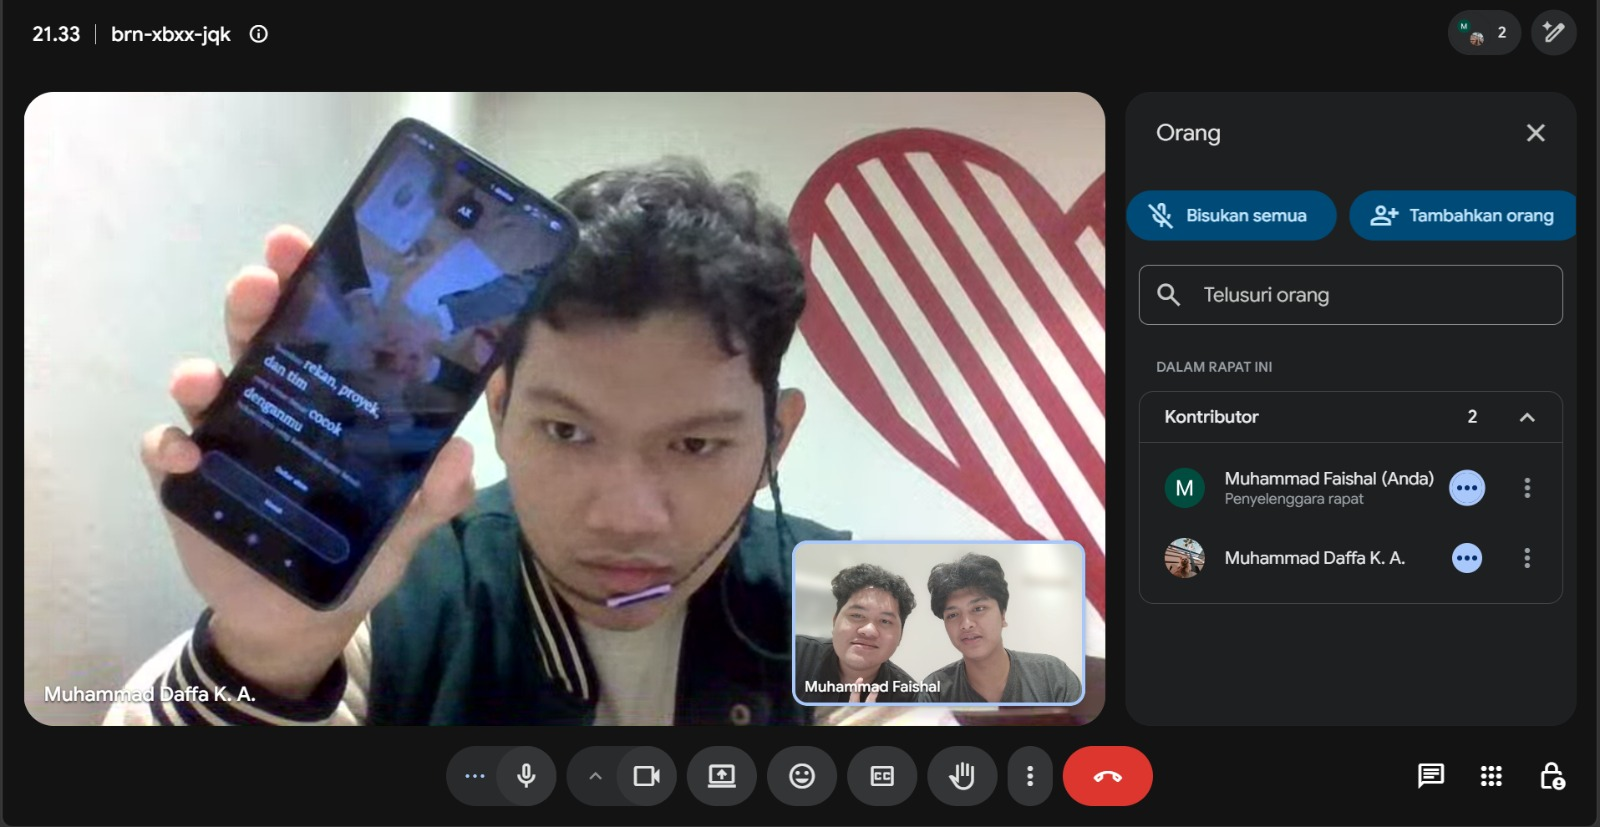
\includegraphics[width=0.75\textwidth]{images/Responden/R5}
  \caption{Dokumentasi Sesi Pengujian bersama Responden 5}
  \label{fig:c-dok5}
\end{figure}

\begin{figure}[H]
  \centering
  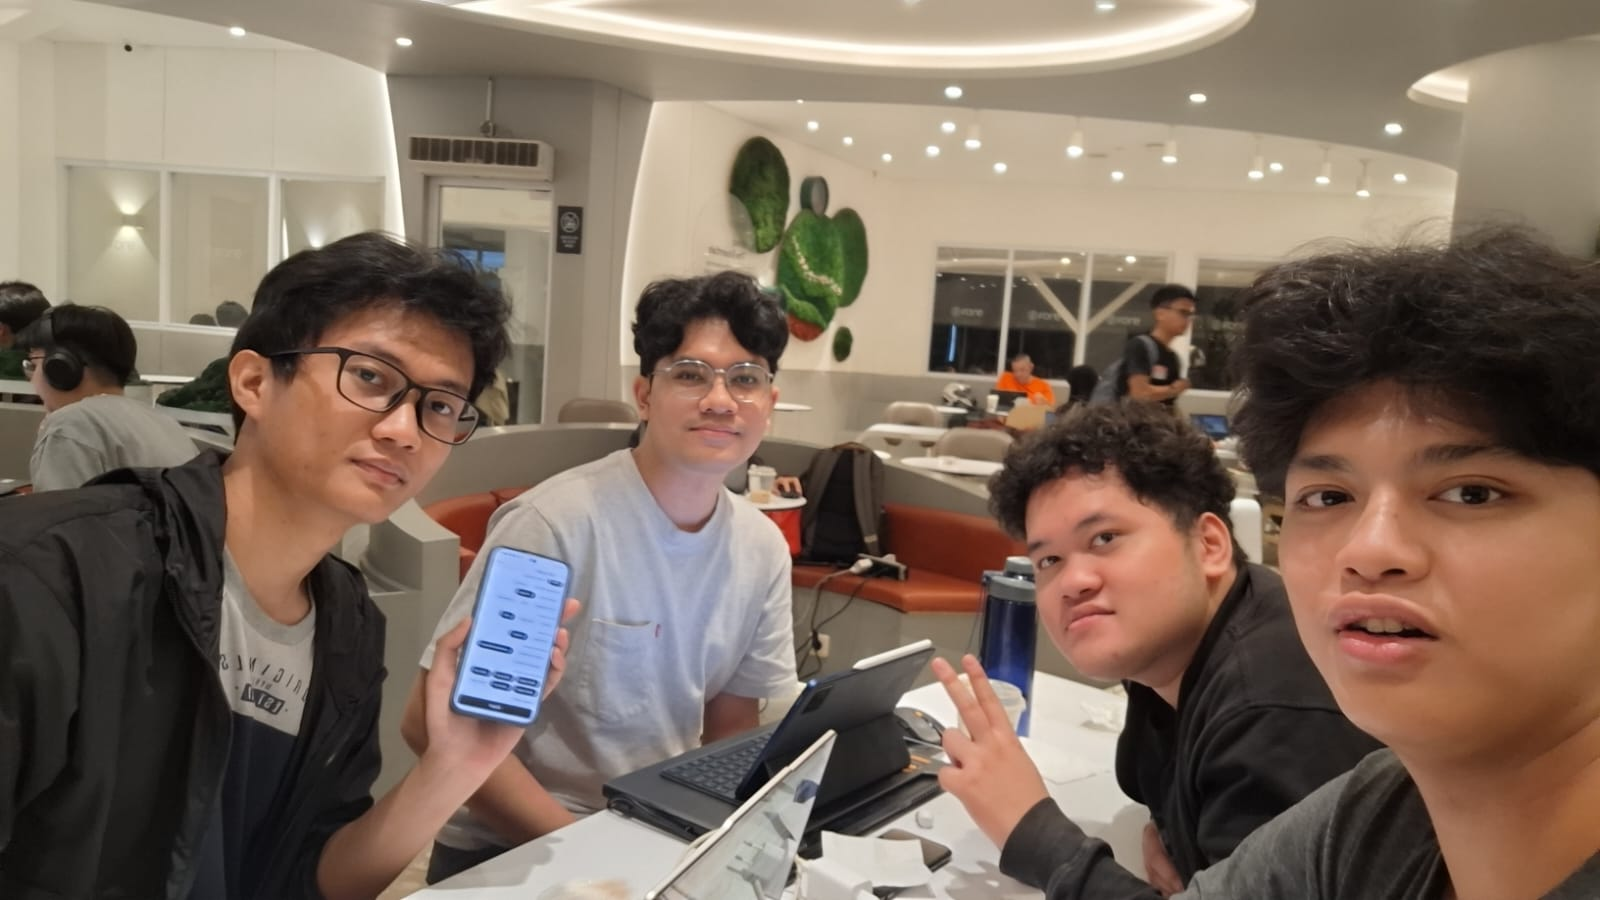
\includegraphics[width=0.85\textwidth]{images/Responden/R67}
  \caption{Dokumentasi Sesi Pengujian bersama Responden 6 dan Responden 7}
  \label{fig:c-dok6}
\end{figure}

\begin{figure}[H]
  \centering
  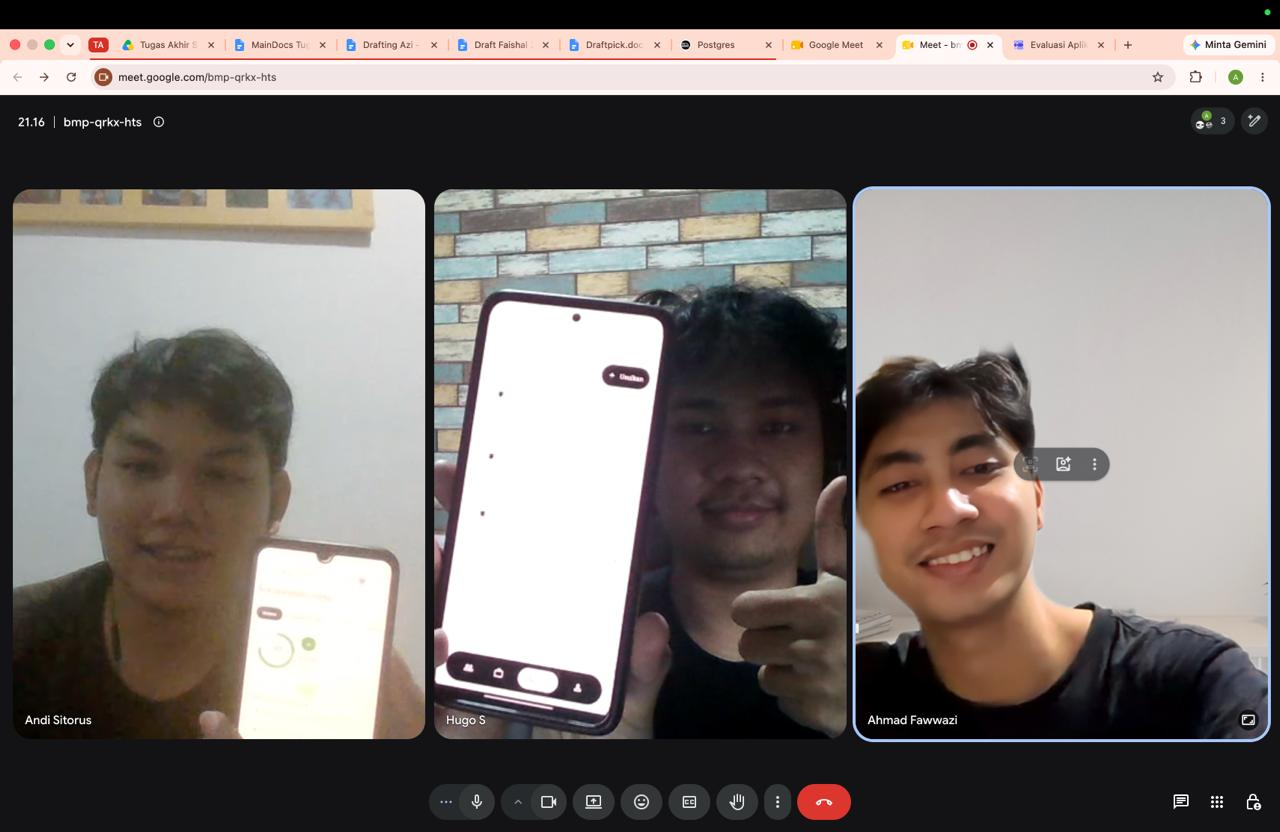
\includegraphics[width=0.85\textwidth]{images/Responden/R89}
  \caption{Dokumentasi Sesi Pengujian bersama Responden 8 dan Responden 9}
  \label{fig:c-dok7}
\end{figure}

\begin{figure}[H]
  \centering
  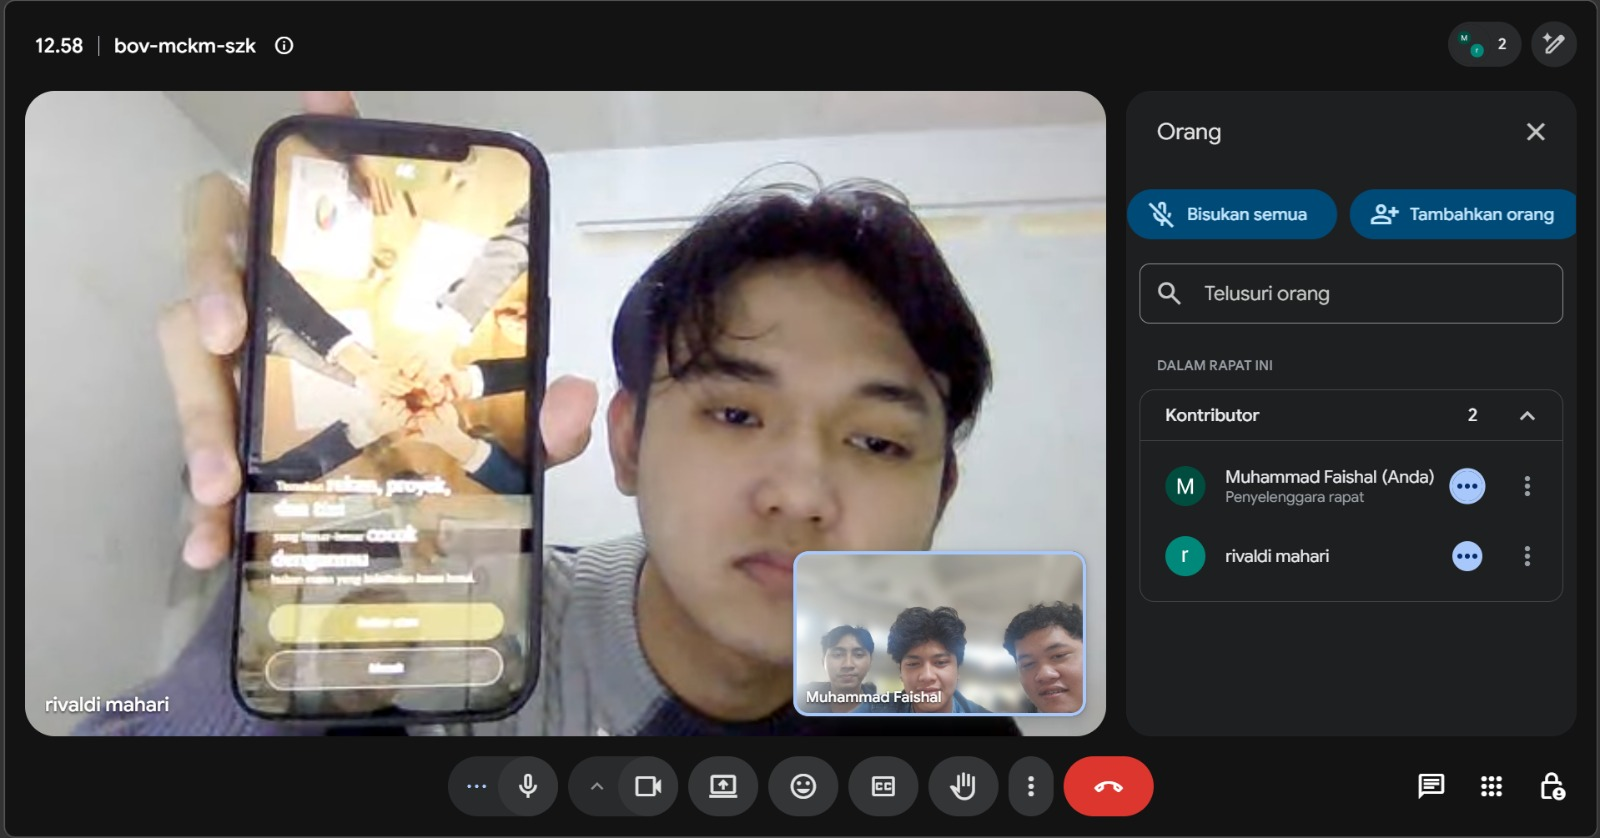
\includegraphics[width=0.85\textwidth]{images/Responden/R10}
  \caption{Dokumentasi Sesi Pengujian bersama Responden 10}
  \label{fig:c-dok8}
\end{figure}
